\section{9 Aprile 2014}
In viaggio per Roma (ESRI Day Auditorium del Massimo ). Questa mattina
mi sono alzato alle 5.00, ho dormito a casa di Annamaria per arrivare
alla stazione più agevolmente. Alle sei ho preso il treno con il mio
collega di sempre Alessandro. Spero che a questa conferenza almeno
ci diano delle indicazione per risolvere un pò di problemi di tecnologia
che abbiamo avuto in questi mesi.

Già da ieri l'applicativo 3Ter Advanced non funziona, ci sono dei
problemi dovuti probabilmente al server LDAP. Nei prossimi giorni
dovremo risolvere questo problema, con Alessandro passeremo le ore
a cercare di risolvere il problema.

Tra oggi e domani devo anche cercare di risolvere il problema dell'intersect
parametrizzato che poi dovrà essere la base per il geoprocessing,
stiamo attendendo ancora i vari parametri da Lukoil. Il difficile
è riuscire a generalizzare uno strumento, cioè andare oltre l'esempio
dei construction sites.

Oramai lavorando in questo campo ho capito che nella parte dei sistemi
è difficilissimo trovare il tuning corretto, soprattutto per le cose
in cui non siamo molto preparati, troppe sono le specificità e a volte
la complessità è molto alta.

Già alle sei ho cominciato a leggere il giornale, mi ha colpito un
articolo sul mancato attacco americano di Agosto 2013, il giornalista
americano sostiene che gli americani non abbiano attaccato perchè
il gas sarin non era effettivamente Siriano ma fosse di alcuni ribelli
jihadisti che per accelerare l'attacco americano avessero utilizzato
gas provenienti dalla Libia tramite la Turchia. Di seguito riporto
il testo in inglese. Io ho letto quello in italiano su laRepubblica,
ma secondo me la traduzione ha qualcosa che non va.

La mattina ho assistito alla sessione plenaria della conferenza ESRI,
nel pomeriggio a delle sessioni tecniche sulle WEB Api e su degli
aspetti geospatial di alcuni software di Business Intelligence. Per
quanto rigurada le web api hanno fatto vedere i nuovi esempi di api
javascript esri, anche con il 3D.

Gli argomenti importanti sono:
\begin{itemize}
\item Sandbox per javascript.
\item SOE java o NET.

\begin{itemize}
\item SOE sono server objects extension sono deployabili in arcgis server
e associabili come capabilities ad ogni servizio del server \Circle{}
Possono essere utilizzate per fare geoprocessing in modo più profondo?
Ma con le arcpy si riesce comunque a costruire strumento di geo-processing.
\end{itemize}
\item Web app builder per creare templates di applicazioni -> funziona solo
con mappe del portale.
\item Nodejs.
\end{itemize}
Nella parte di business intelligence il GIS alla fine è soltanto uno
strumento che visualizza i risultati di elaborazioni più complesse.
Tuttavia ci sono applicazione di geomarketing molto più complesse
che al loro interno hanno degli algoritmi molto più complessi.

La sera ho cenato con i miei colleghi, abbiamo discusso dell'azienda
e del lavoro facendo emergere le solite problematiche legate alle
solite persone e legate alla dirigenza che ha una bassa percezione
del problema organizzativo.


\subsection{The Red Line and the Rat Line}

\url{http://www.lrb.co.uk/v36/n08/seymour-m-hersh/the-red-line-and-the-rat-line}


\subsubsection{Seymour M. Hersh on Obama, Erdo\u{g}an and the Syrian rebels}

In 2011 Barack Obama led an allied military intervention in Libya
without consulting the US Congress. Last August, after the sarin attack
on the Damascus suburb of Ghouta, he was ready to launch an allied
air strike, this time to punish the Syrian government for allegedly
crossing the 'red line' he had set in 2012 on the use of chemical
weapons. Then with less than two days to go before the planned strike,
he announced that he would seek congressional approval for the intervention.
The strike was postponed as Congress prepared for hearings, and subsequently
cancelled when Obama accepted Assad's offer to relinquish his chemical
arsenal in a deal brokered by Russia. Why did Obama delay and then
relent on Syria when he was not shy about rushing into Libya? The
answer lies in a clash between those in the administration who were
committed to enforcing the red line, and military leaders who thought
that going to war was both unjustified and potentially disastrous.

Obama's change of mind had its origins at Porton Down, the defence
laboratory in Wiltshire. British intelligence had obtained a sample
of the sarin used in the 21 August attack and analysis demonstrated
that the gas used didn't match the batches known to exist in the Syrian
army's chemical weapons arsenal. The message that the case against
Syria wouldn't hold up was quickly relayed to the US joint chiefs
of staff. The British report heightened doubts inside the Pentagon;
the joint chiefs were already preparing to warn Obama that his plans
for a far-reaching bomb and missile attack on Syria's infrastructure
could lead to a wider war in the Middle East. As a consequence the
American officers delivered a last-minute caution to the president,
which, in their view, eventually led to his cancelling the attack.

For months there had been acute concern among senior military leaders
and the intelligence community about the role in the war of Syria's
neighbours, especially Turkey. Prime Minister Recep Erdo\u{g}an was
known to be supporting the al-Nusra Front, a jihadist faction among
the rebel opposition, as well as other Islamist rebel groups. 'We
knew there were some in the Turkish government,' a former senior US
intelligence official, who has access to current intelligence, told
me, 'who believed they could get Assad's nuts in a vice by dabbling
with a sarin attack inside Syria \textendash{} and forcing Obama to
make good on his red line threat.'

The joint chiefs also knew that the Obama administration's public
claims that only the Syrian army had access to sarin were wrong. The
American and British intelligence communities had been aware since
the spring of 2013 that some rebel units in Syria were developing
chemical weapons. On 20 June analysts for the US Defense Intelligence
Agency issued a highly classified five-page 'talking points' briefing
for the DIA's deputy director, David Shedd, which stated that al-Nusra
maintained a sarin production cell: its programme, the paper said,
was 'the most advanced sarin plot since al-Qaida's pre-9/11 effort'.
(According to a Defense Department consultant, US intelligence has
long known that al-Qaida experimented with chemical weapons, and has
a video of one of its gas experiments with dogs.) The DIA paper went
on: 'Previous IC {[}intelligence community{]} focus had been almost
entirely on Syrian CW {[}chemical weapons{]} stockpiles; now we see
ANF attempting to make its own CW \ldots{} Al-Nusrah Front's relative
freedom of operation within Syria leads us to assess the group's CW
aspirations will be difficult to disrupt in the future.' The paper
drew on classified intelligence from numerous agencies: 'Turkey and
Saudi-based chemical facilitators,' it said, 'were attempting to obtain
sarin precursors in bulk, tens of kilograms, likely for the anticipated
large scale production effort in Syria.' (Asked about the DIA paper,
a spokesperson for the director of national intelligence said: 'No
such paper was ever requested or produced by intelligence community
analysts.')

Last May, more than ten members of the al-Nusra Front were arrested
in southern Turkey with what local police told the press were two
kilograms of sarin. In a 130-page indictment the group was accused
of attempting to purchase fuses, piping for the construction of mortars,
and chemical precursors for sarin. Five of those arrested were freed
after a brief detention. The others, including the ringleader, Haytham
Qassab, for whom the prosecutor requested a prison sentence of 25
years, were released pending trial. In the meantime the Turkish press
has been rife with speculation that the Erdo\u{g}an administration
has been covering up the extent of its involvement with the rebels.
In a news conference last summer, Aydin Sezgin, Turkey's ambassador
to Moscow, dismissed the arrests and claimed to reporters that the
recovered 'sarin' was merely 'anti-freeze'.

The DIA paper took the arrests as evidence that al-Nusra was expanding
its access to chemical weapons. It said Qassab had 'self-identified'
as a member of al-Nusra, and that he was directly connected to Abd-al-Ghani,
the 'ANF emir for military manufacturing'. Qassab and his associate
Khalid Ousta worked with Halit Unalkaya, an employee of a Turkish
firm called Zirve Export, who provided 'price quotes for bulk quantities
of sarin precursors'. Abd-al-Ghani's plan was for two associates to
'perfect a process for making sarin, then go to Syria to train others
to begin large scale production at an unidentified lab in Syria'.
The DIA paper said that one of his operatives had purchased a precursor
on the 'Baghdad chemical market', which 'has supported at least seven
CW efforts since 2004'.

A series of chemical weapon attacks in March and April 2013 was investigated
over the next few months by a special UN mission to Syria. A person
with close knowledge of the UN's activity in Syria told me that there
was evidence linking the Syrian opposition to the first gas attack,
on 19 March in Khan Al-Assal, a village near Aleppo. In its final
report in December, the mission said that at least 19 civilians and
one Syrian soldier were among the fatalities, along with scores of
injured. It had no mandate to assign responsibility for the attack,
but the person with knowledge of the UN's activities said: 'Investigators
interviewed the people who were there, including the doctors who treated
the victims. It was clear that the rebels used the gas. It did not
come out in public because no one wanted to know.'

In the months before the attacks began, a former senior Defense Department
official told me, the DIA was circulating a daily classified report
known as SYRUP on all intelligence related to the Syrian conflict,
including material on chemical weapons. But in the spring, distribution
of the part of the report concerning chemical weapons was severely
curtailed on the orders of Denis McDonough, the White House chief
of staff. 'Something was in there that triggered a shit fit by McDonough,'
the former Defense Department official said. 'One day it was a huge
deal, and then, after the March and April sarin attacks' \textendash{}
he snapped his fingers \textendash{} 'it's no longer there.' The decision
to restrict distribution was made as the joint chiefs ordered intensive
contingency planning for a possible ground invasion of Syria whose
primary objective would be the elimination of chemical weapons.

The former intelligence official said that many in the US national
security establishment had long been troubled by the president's red
line: 'The joint chiefs asked the White House, ``What does red line
mean? How does that translate into military orders? Troops on the
ground? Massive strike? Limited strike?'' They tasked military intelligence
to study how we could carry out the threat. They learned nothing more
about the president's reasoning.'

In the aftermath of the 21 August attack Obama ordered the Pentagon
to draw up targets for bombing. Early in the process, the former intelligence
official said, 'the White House rejected 35 target sets provided by
the joint chiefs of staff as being insufficiently \textquotedbl{}painful\textquotedbl{}
to the Assad regime.' The original targets included only military
sites and nothing by way of civilian infrastructure. Under White House
pressure, the US attack plan evolved into 'a monster strike': two
wings of B-52 bombers were shifted to airbases close to Syria, and
navy submarines and ships equipped with Tomahawk missiles were deployed.
'Every day the target list was getting longer,' the former intelligence
official told me. 'The Pentagon planners said we can't use only Tomahawks
to strike at Syria's missile sites because their warheads are buried
too far below ground, so the two B-52 air wings with two-thousand
pound bombs were assigned to the mission. Then we'll need standby
search-and-rescue teams to recover downed pilots and drones for target
selection. It became huge.' The new target list was meant to 'completely
eradicate any military capabilities Assad had', the former intelligence
official said. The core targets included electric power grids, oil
and gas depots, all known logistic and weapons depots, all known command
and control facilities, and all known military and intelligence buildings.

Britain and France were both to play a part. On 29 August, the day
Parliament voted against Cameron's bid to join the intervention, the
Guardian reported that he had already ordered six RAF Typhoon fighter
jets to be deployed to Cyprus, and had volunteered a submarine capable
of launching Tomahawk missiles. The French air force \textendash{}
a crucial player in the 2011 strikes on Libya \textendash{} was deeply
committed, according to an account in Le Nouvel Observateur; François
Hollande had ordered several Rafale fighter-bombers to join the American
assault. Their targets were reported to be in western Syria.

By the last days of August the president had given the Joint Chiefs
a fixed deadline for the launch. 'H hour was to begin no later than
Monday morning {[}2 September{]}, a massive assault to neutralise
Assad,' the former intelligence official said. So it was a surprise
to many when during a speech in the White House Rose Garden on 31
August Obama said that the attack would be put on hold, and he would
turn to Congress and put it to a vote.

At this stage, Obama's premise \textendash{} that only the Syrian
army was capable of deploying sarin \textendash{} was unravelling.
Within a few days of the 21 August attack, the former intelligence
official told me, Russian military intelligence operatives had recovered
samples of the chemical agent from Ghouta. They analysed it and passed
it on to British military intelligence; this was the material sent
to Porton Down. (A spokesperson for Porton Down said: 'Many of the
samples analysed in the UK tested positive for the nerve agent sarin.'
MI6 said that it doesn't comment on intelligence matters.)

The former intelligence official said the Russian who delivered the
sample to the UK was 'a good source \textendash{} someone with access,
knowledge and a record of being trustworthy'. After the first reported
uses of chemical weapons in Syria last year, American and allied intelligence
agencies 'made an effort to find the answer as to what if anything,
was used \textendash{} and its source', the former intelligence official
said. 'We use data exchanged as part of the Chemical Weapons Convention.
The DIA's baseline consisted of knowing the composition of each batch
of Soviet-manufactured chemical weapons. But we didn't know which
batches the Assad government currently had in its arsenal. Within
days of the Damascus incident we asked a source in the Syrian government
to give us a list of the batches the government currently had. This
is why we could confirm the difference so quickly.'

The process hadn't worked as smoothly in the spring, the former intelligence
official said, because the studies done by Western intelligence 'were
inconclusive as to the type of gas it was. The word ``sarin'' didn't
come up. There was a great deal of discussion about this, but since
no one could conclude what gas it was, you could not say that Assad
had crossed the president's red line.' By 21 August, the former intelligence
official went on, 'the Syrian opposition clearly had learned from
this and announced that \textquotedbl{}sarin\textquotedbl{} from the
Syrian army had been used, before any analysis could be made, and
the press and White House jumped at it. Since it now was sarin, \textquotedbl{}It
had to be Assad.\textquotedbl{}'

The UK defence staff who relayed the Porton Down findings to the joint
chiefs were sending the Americans a message, the former intelligence
official said: 'We're being set up here.' (This account made sense
of a terse message a senior official in the CIA sent in late August:
'It was not the result of the current regime. UK \& US know this.')
By then the attack was a few days away and American, British and French
planes, ships and submarines were at the ready.

The officer ultimately responsible for the planning and execution
of the attack was General Martin Dempsey, chairman of the joint chiefs.
From the beginning of the crisis, the former intelligence official
said, the joint chiefs had been sceptical of the administration's
argument that it had the facts to back up its belief in Assad's guilt.
They pressed the DIA and other agencies for more substantial evidence.
'There was no way they thought Syria would use nerve gas at that stage,
because Assad was winning the war,' the former intelligence official
said. Dempsey had irritated many in the Obama administration by repeatedly
warning Congress over the summer of the danger of American military
involvement in Syria. Last April, after an optimistic assessment of
rebel progress by the secretary of state, John Kerry, in front of
the House Foreign Affairs Committee, Dempsey told the Senate Armed
Services Committee that 'there's a risk that this conflict has become
stalemated.'

Dempsey's initial view after 21 August was that a US strike on Syria
\textendash{} under the assumption that the Assad government was responsible
for the sarin attack \textendash{} would be a military blunder, the
former intelligence official said. The Porton Down report caused the
joint chiefs to go to the president with a more serious worry: that
the attack sought by the White House would be an unjustified act of
aggression. It was the joint chiefs who led Obama to change course.
The official White House explanation for the turnabout \textendash{}
the story the press corps told \textendash{} was that the president,
during a walk in the Rose Garden with Denis McDonough, his chief of
staff, suddenly decided to seek approval for the strike from a bitterly
divided Congress with which he'd been in conflict for years. The former
Defense Department official told me that the White House provided
a different explanation to members of the civilian leadership of the
Pentagon: the bombing had been called off because there was intelligence
'that the Middle East would go up in smoke' if it was carried out.

The president's decision to go to Congress was initially seen by senior
aides in the White House, the former intelligence official said, as
a replay of George W. Bush's gambit in the autumn of 2002 before the
invasion of Iraq: 'When it became clear that there were no WMD in
Iraq, Congress, which had endorsed the Iraqi war, and the White House
both shared the blame and repeatedly cited faulty intelligence. If
the current Congress were to vote to endorse the strike, the White
House could again have it both ways \textendash{} wallop Syria with
a massive attack and validate the president's red line commitment,
while also being able to share the blame with Congress if it came
out that the Syrian military wasn't behind the attack.' The turnabout
came as a surprise even to the Democratic leadership in Congress.
In September the Wall Street Journal reported that three days before
his Rose Garden speech Obama had telephoned Nancy Pelosi, leader of
the House Democrats, 'to talk through the options'. She later told
colleagues, according to the Journal, that she hadn't asked the president
to put the bombing to a congressional vote.

Obama's move for congressional approval quickly became a dead end.
'Congress was not going to let this go by,' the former intelligence
official said. 'Congress made it known that, unlike the authorisation
for the Iraq war, there would be substantive hearings.' At this point,
there was a sense of desperation in the White House, the former intelligence
official said. 'And so out comes Plan B. Call off the bombing strike
and Assad would agree to unilaterally sign the chemical warfare treaty
and agree to the destruction of all of chemical weapons under UN supervision.'
At a press conference in London on 9 September, Kerry was still talking
about intervention: 'The risk of not acting is greater than the risk
of acting.' But when a reporter asked if there was anything Assad
could do to stop the bombing, Kerry said: 'Sure. He could turn over
every single bit of his chemical weapons to the international community
in the next week \ldots{} But he isn't about to do it, and it can't
be done, obviously.' As the New York Times reported the next day,
the Russian-brokered deal that emerged shortly afterwards had first
been discussed by Obama and Putin in the summer of 2012. Although
the strike plans were shelved, the administration didn't change its
public assessment of the justification for going to war. 'There is
zero tolerance at that level for the existence of error,' the former
intelligence official said of the senior officials in the White House.
'They could not afford to say: \textquotedbl{}We were wrong.\textquotedbl{}'
(The DNI spokesperson said: 'The Assad regime, and only the Assad
regime, could have been responsible for the chemical weapons attack
that took place on 21 August.')

{*}

The full extent of US co-operation with Turkey, Saudi Arabia and Qatar
in assisting the rebel opposition in Syria has yet to come to light.
The Obama administration has never publicly admitted to its role in
creating what the CIA calls a 'rat line', a back channel highway into
Syria. The rat line, authorised in early 2012, was used to funnel
weapons and ammunition from Libya via southern Turkey and across the
Syrian border to the opposition. Many of those in Syria who ultimately
received the weapons were jihadists, some of them affiliated with
al-Qaida. (The DNI spokesperson said: 'The idea that the United States
was providing weapons from Libya to anyone is false.')

In January, the Senate Intelligence Committee released a report on
the assault by a local militia in September 2012 on the American consulate
and a nearby undercover CIA facility in Benghazi, which resulted in
the death of the US ambassador, Christopher Stevens, and three others.
The report's criticism of the State Department for not providing adequate
security at the consulate, and of the intelligence community for not
alerting the US military to the presence of a CIA outpost in the area,
received front-page coverage and revived animosities in Washington,
with Republicans accusing Obama and Hillary Clinton of a cover-up.
A highly classified annex to the report, not made public, described
a secret agreement reached in early 2012 between the Obama and Erdo\u{g}an
administrations. It pertained to the rat line. By the terms of the
agreement, funding came from Turkey, as well as Saudi Arabia and Qatar;
the CIA, with the support of MI6, was responsible for getting arms
from Gaddafi's arsenals into Syria. A number of front companies were
set up in Libya, some under the cover of Australian entities. Retired
American soldiers, who didn't always know who was really employing
them, were hired to manage procurement and shipping. The operation
was run by David Petraeus, the CIA director who would soon resign
when it became known he was having an affair with his biographer.
(A spokesperson for Petraeus denied the operation ever took place.)

The operation had not been disclosed at the time it was set up to
the congressional intelligence committees and the congressional leadership,
as required by law since the 1970s. The involvement of MI6 enabled
the CIA to evade the law by classifying the mission as a liaison operation.
The former intelligence official explained that for years there has
been a recognised exception in the law that permits the CIA not to
report liaison activity to Congress, which would otherwise be owed
a finding. (All proposed CIA covert operations must be described in
a written document, known as a 'finding', submitted to the senior
leadership of Congress for approval.) Distribution of the annex was
limited to the staff aides who wrote the report and to the eight ranking
members of Congress \textendash{} the Democratic and Republican leaders
of the House and Senate, and the Democratic and Republicans leaders
on the House and Senate intelligence committees. This hardly constituted
a genuine attempt at oversight: the eight leaders are not known to
gather together to raise questions or discuss the secret information
they receive.

The annex didn't tell the whole story of what happened in Benghazi
before the attack, nor did it explain why the American consulate was
attacked. 'The consulate's only mission was to provide cover for the
moving of arms,' the former intelligence official, who has read the
annex, said. 'It had no real political role.'

Washington abruptly ended the CIA's role in the transfer of arms from
Libya after the attack on the consulate, but the rat line kept going.
'The United States was no longer in control of what the Turks were
relaying to the jihadists,' the former intelligence official said.
Within weeks, as many as forty portable surface-to-air missile launchers,
commonly known as manpads, were in the hands of Syrian rebels. On
28 November 2012, Joby Warrick of the Washington Post reported that
the previous day rebels near Aleppo had used what was almost certainly
a manpad to shoot down a Syrian transport helicopter. 'The Obama administration,'
Warrick wrote, 'has steadfastly opposed arming Syrian opposition forces
with such missiles, warning that the weapons could fall into the hands
of terrorists and be used to shoot down commercial aircraft.' Two
Middle Eastern intelligence officials fingered Qatar as the source,
and a former US intelligence analyst speculated that the manpads could
have been obtained from Syrian military outposts overrun by the rebels.
There was no indication that the rebels' possession of manpads was
likely the unintended consequence of a covert US programme that was
no longer under US control.

By the end of 2012, it was believed throughout the American intelligence
community that the rebels were losing the war. 'Erdo\u{g}an was pissed,'
the former intelligence official said, 'and felt he was left hanging
on the vine. It was his money and the cut-off was seen as a betrayal.'
In spring 2013 US intelligence learned that the Turkish government
\textendash{} through elements of the MIT, its national intelligence
agency, and the Gendarmerie, a militarised law-enforcement organisation
\textendash{} was working directly with al-Nusra and its allies to
develop a chemical warfare capability. 'The MIT was running the political
liaison with the rebels, and the Gendarmerie handled military logistics,
on-the-scene advice and training \textendash{} including training
in chemical warfare,' the former intelligence official said. 'Stepping
up Turkey's role in spring 2013 was seen as the key to its problems
there. Erdo\u{g}an knew that if he stopped his support of the jihadists
it would be all over. The Saudis could not support the war because
of logistics \textendash{} the distances involved and the difficulty
of moving weapons and supplies. Erdo\u{g}an's hope was to instigate
an event that would force the US to cross the red line. But Obama
didn't respond in March and April.'

There was no public sign of discord when Erdo\u{g}an and Obama met
on 16 May 2013 at the White House. At a later press conference Obama
said that they had agreed that Assad 'needs to go'. Asked whether
he thought Syria had crossed the red line, Obama acknowledged that
there was evidence such weapons had been used, but added, 'it is important
for us to make sure that we're able to get more specific information
about what exactly is happening there.' The red line was still intact.

An American foreign policy expert who speaks regularly with officials
in Washington and Ankara told me about a working dinner Obama held
for Erdo\u{g}an during his May visit. The meal was dominated by the
Turks' insistence that Syria had crossed the red line and their complaints
that Obama was reluctant to do anything about it. Obama was accompanied
by John Kerry and Tom Donilon, the national security adviser who would
soon leave the job. Erdo\u{g}an was joined by Ahmet Davuto\u{g}lu,
Turkey's foreign minister, and Hakan Fidan, the head of the MIT. Fidan
is known to be fiercely loyal to Erdo\u{g}an, and has been seen as
a consistent backer of the radical rebel opposition in Syria.

The foreign policy expert told me that the account he heard originated
with Donilon. (It was later corroborated by a former US official,
who learned of it from a senior Turkish diplomat.) According to the
expert, Erdo\u{g}an had sought the meeting to demonstrate to Obama
that the red line had been crossed, and had brought Fidan along to
state the case. When Erdo\u{g}an tried to draw Fidan into the conversation,
and Fidan began speaking, Obama cut him off and said: 'We know.' Erdo\u{g}an
tried to bring Fidan in a second time, and Obama again cut him off
and said: 'We know.' At that point, an exasperated Erdo\u{g}an said,
'But your red line has been crossed!' and, the expert told me, 'Donilon
said Erdo\u{g}an \textquotedbl{}fucking waved his finger at the president
inside the White House\textquotedbl{}.' Obama then pointed at Fidan
and said: 'We know what you're doing with the radicals in Syria.'
(Donilon, who joined the Council on Foreign Relations last July, didn't
respond to questions about this story. The Turkish Foreign Ministry
didn't respond to questions about the dinner. A spokesperson for the
National Security Council confirmed that the dinner took place and
provided a photograph showing Obama, Kerry, Donilon, Erdo\u{g}an,
Fidan and Davuto\u{g}lu sitting at a table. 'Beyond that,' she said,
'I'm not going to read out the details of their discussions.')

But Erdo\u{g}an did not leave empty handed. Obama was still permitting
Turkey to continue to exploit a loophole in a presidential executive
order prohibiting the export of gold to Iran, part of the US sanctions
regime against the country. In March 2012, responding to sanctions
of Iranian banks by the EU, the SWIFT electronic payment system, which
facilitates cross-border payments, expelled dozens of Iranian financial
institutions, severely restricting the country's ability to conduct
international trade. The US followed with the executive order in July,
but left what came to be known as a 'golden loophole': gold shipments
to private Iranian entities could continue. Turkey is a major purchaser
of Iranian oil and gas, and it took advantage of the loophole by depositing
its energy payments in Turkish lira in an Iranian account in Turkey;
these funds were then used to purchase Turkish gold for export to
confederates in Iran. Gold to the value of \$13 billion reportedly
entered Iran in this way between March 2012 and July 2013.

The programme quickly became a cash cow for corrupt politicians and
traders in Turkey, Iran and the United Arab Emirates. 'The middlemen
did what they always do,' the former intelligence official said. 'Take
15 per cent. The CIA had estimated that there was as much as two billion
dollars in skim. Gold and Turkish lira were sticking to fingers.'
The illicit skimming flared into a public 'gas for gold' scandal in
Turkey in December, and resulted in charges against two dozen people,
including prominent businessmen and relatives of government officials,
as well as the resignations of three ministers, one of whom called
for Erdo\u{g}an to resign. The chief executive of a Turkish state-controlled
bank that was in the middle of the scandal insisted that more than
\$4.5 million in cash found by police in shoeboxes during a search
of his home was for charitable donations.

Late last year Jonathan Schanzer and Mark Dubowitz reported in Foreign
Policy that the Obama administration closed the golden loophole in
January 2013, but 'lobbied to make sure the legislation \ldots{} did
not take effect for six months'. They speculated that the administration
wanted to use the delay as an incentive to bring Iran to the bargaining
table over its nuclear programme, or to placate its Turkish ally in
the Syrian civil war. The delay permitted Iran to 'accrue billions
of dollars more in gold, further undermining the sanctions regime'.

{*}

The American decision to end CIA support of the weapons shipments
into Syria left Erdo\u{g}an exposed politically and militarily. 'One
of the issues at that May summit was the fact that Turkey is the only
avenue to supply the rebels in Syria,' the former intelligence official
said. 'It can't come through Jordan because the terrain in the south
is wide open and the Syrians are all over it. And it can't come through
the valleys and hills of Lebanon \textendash{} you can't be sure who
you'd meet on the other side.' Without US military support for the
rebels, the former intelligence official said, 'Erdo\u{g}an's dream
of having a client state in Syria is evaporating and he thinks we're
the reason why. When Syria wins the war, he knows the rebels are just
as likely to turn on him \textendash{} where else can they go? So
now he will have thousands of radicals in his backyard.'

A US intelligence consultant told me that a few weeks before 21 August
he saw a highly classified briefing prepared for Dempsey and the defense
secretary, Chuck Hagel, which described 'the acute anxiety' of the
Erdo\u{g}an administration about the rebels' dwindling prospects.
The analysis warned that the Turkish leadership had expressed 'the
need to do something that would precipitate a US military response'.
By late summer, the Syrian army still had the advantage over the rebels,
the former intelligence official said, and only American air power
could turn the tide. In the autumn, the former intelligence official
went on, the US intelligence analysts who kept working on the events
of 21 August 'sensed that Syria had not done the gas attack. But the
500 pound gorilla was, how did it happen? The immediate suspect was
the Turks, because they had all the pieces to make it happen.'

As intercepts and other data related to the 21 August attacks were
gathered, the intelligence community saw evidence to support its suspicions.
'We now know it was a covert action planned by Erdo\u{g}an's people
to push Obama over the red line,' the former intelligence official
said. 'They had to escalate to a gas attack in or near Damascus when
the UN inspectors' \textendash{} who arrived in Damascus on 18 August
to investigate the earlier use of gas \textendash{} 'were there. The
deal was to do something spectacular. Our senior military officers
have been told by the DIA and other intelligence assets that the sarin
was supplied through Turkey \textendash{} that it could only have
gotten there with Turkish support. The Turks also provided the training
in producing the sarin and handling it.' Much of the support for that
assessment came from the Turks themselves, via intercepted conversations
in the immediate aftermath of the attack. 'Principal evidence came
from the Turkish post-attack joy and back-slapping in numerous intercepts.
Operations are always so super-secret in the planning but that all
flies out the window when it comes to crowing afterwards. There is
no greater vulnerability than in the perpetrators claiming credit
for success.' Erdo\u{g}an's problems in Syria would soon be over:
'Off goes the gas and Obama will say red line and America is going
to attack Syria, or at least that was the idea. But it did not work
out that way.'

The post-attack intelligence on Turkey did not make its way to the
White House. 'Nobody wants to talk about all this,' the former intelligence
official told me. 'There is great reluctance to contradict the president,
although no all-source intelligence community analysis supported his
leap to convict. There has not been one single piece of additional
evidence of Syrian involvement in the sarin attack produced by the
White House since the bombing raid was called off. My government can't
say anything because we have acted so irresponsibly. And since we
blamed Assad, we can't go back and blame Erdo\u{g}an.'

Turkey's willingness to manipulate events in Syria to its own purposes
seemed to be demonstrated late last month, a few days before a round
of local elections, when a recording, allegedly of Erdo\u{g}an and
his associates, was posted to YouTube. It included discussion of a
false-flag operation that would justify an incursion by the Turkish
military in Syria. The operation centred on the tomb of Suleyman Shah,
the grandfather of the revered Osman I, founder of the Ottoman Empire,
which is near Aleppo and was ceded to Turkey in 1921, when Syria was
under French rule. One of the Islamist rebel factions was threatening
to destroy the tomb as a site of idolatry, and the Erdo\u{g}an administration
was publicly threatening retaliation if harm came to it. According
to a Reuters report of the leaked conversation, a voice alleged to
be Fidan's spoke of creating a provocation: 'Now look, my commander
{[}Erdo\u{g}an{]}, if there is to be justification, the justification
is I send four men to the other side. I get them to fire eight missiles
into empty land {[}in the vicinity of the tomb{]}. That's not a problem.
Justification can be created.' The Turkish government acknowledged
that there had been a national security meeting about threats emanating
from Syria, but said the recording had been manipulated. The government
subsequently blocked public access to YouTube.

Barring a major change in policy by Obama, Turkey's meddling in the
Syrian civil war is likely to go on. 'I asked my colleagues if there
was any way to stop Erdo\u{g}an's continued support for the rebels,
especially now that it's going so wrong,' the former intelligence
official told me. 'The answer was: \textquotedbl{}We're screwed.\textquotedbl{}
We could go public if it was somebody other than Erdo\u{g}an, but
Turkey is a special case. They're a Nato ally. The Turks don't trust
the West. They can't live with us if we take any active role against
Turkish interests. If we went public with what we know about Erdo\u{g}an's
role with the gas, it'd be disastrous. The Turks would say: ``We
hate you for telling us what we can and can't do.''


\section{10 Aprile 2014}

Questa mattina mi sono svegliato più volte a partire dalle cinque
del mattino, alle sette e mezzo mi sono alzato, lavato e sono andato
a fare colazione. Negli alberghi di Roma non sono mai riuscito a fare
una colazione decente, sempre bicchieri di carta, ma sopratutto cibo
un pò scadente. Comunque Roma rimane più bella e più attraente di
Milano. La giornata è passata alla conferenza, ho ritrovato l'amico
Renzo Carlucci e Domenico Santarsiero. Loro lavoravano con me in Siria,
al progetto della cooperazione Italiana. Ho tanti ricordi di quella esperienza in Siria tutti molto belli. Stare in quel paese per me è stata una rivelazione, ho conosciuto cose di cui ignoravo l'esistenza. Troppo è il dolore che sto provando in questi ultimi due anni, per la situazione che si sta delineando in quel paese. Fame, morte e distruzione. Inoltre di padre Dall'Oglio non sia hanno più notizie; lo conobbi a Deir Mar Musa nel suo conv ento/eremo. Un posto fantastico e suggestivo con dei mosaici di centinaia di anni.
\begin{figure}[!htbp]
 \centering
 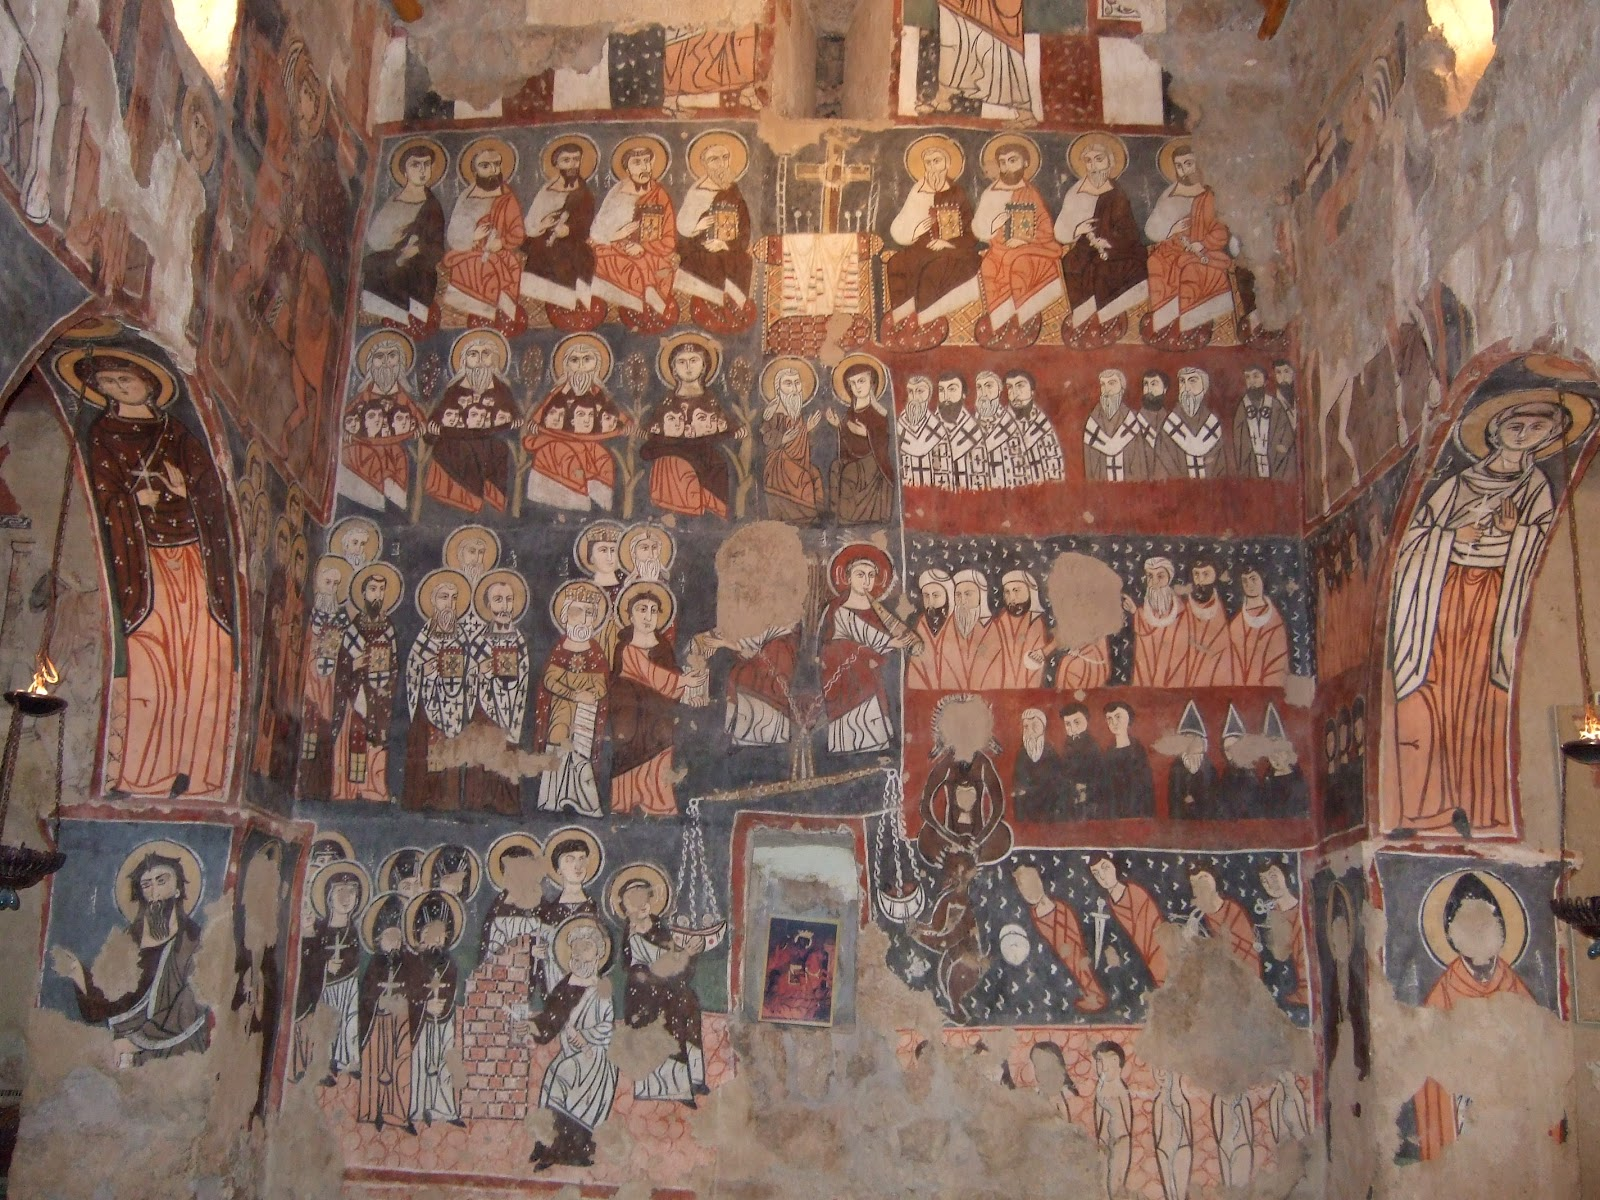
\includegraphics[width=\linewidth]{DSCF0274.jpg}
 \caption{Muro Est, "Il Giudizio Universale"}
\end{figure}


Ricordo che padre Paolo sosteneva che all'interno del monastero vi fosse un'antica porta che portava ad altri locali usati dai monaci nell'atichità.
Dopo la conferenza ho preso il treno con Alessandro e sono tornato a casa da Annamaria. Ho mangiato e poi sono andato a dormire. Annamaria si è anche arrabbiata con me perchè gli ho risposto male, mi sono innervosito perchè non voleva mettere la tovaglia, dopo ci siamo riappacificati e siamo andati a dormire.
\section{14 Aprile 2014}
Oggi è lunedì, con difficoltà mi sono alzato. Ultimamente non riesco ad alzarmi presto se non con grande sforzo, secondo me è l'ora legale e la diminuzione degli allenamenti. Ieri sera ho visto il nome della rosa, l'ultima volta che lo avevo visto avevo 18 anni. Oggi mi sono preso l'ebook che credo leggerò già da stasera.\\
Per tutto il giorno sono stato in ufficio a lavorare sul progetto lukoil, che spero di portare a termine senza danni;
 comunque uno dei miei desideri più grandi è andarmene da questa azienda e possibilmente da questa città, portandomi via anche Annamaria. Sto riflettendo sul fatto di inviare il curriculum vitae al nostro principale concorrente. Perchè non dovrei farlo? In fin dei conti non sono libero di andare a lavorare dove voglio? Credo che lo farò senza grosse remore, solo che potrei mettermi in una posizione critica. Nel nostro ufficio Overit è considerata come il nemico numero uno, forse esagerando. Anche se anche io credo che loro abbiano degli aiuti da parte di SRG.\\
In GESP sembra che tutti siano amici, dopo tra loro si parlano alle spalle oppure si mettono i bastoni tra le ruote nel lavoro. E' penoso che questo accada in un ambiente lavorativo, non porta a nulla e porta all'isolamento e alla formazione di fazioni interne all'azienda. Io ed Annamaria tendiamo a farci gli affari nostri in modo molto diplomatico.\par
Spesso mi capita di vedere un giorno in pretura, in molti mi prendono in giro per questo. Ma sono convinto di una cosa che guardandolo una persona può farsi un'idea delle piaghe della civiltà in cui viviamo, certo è vero che i delitti ci sono sempre stati e sempre ci saranno. Ma in questo caso bisogna saper guardare a ciò che è indotto dalla società e della brama di denaro (omicidio Igor Franchini) piuttosto che al delitto dovuto all'ignoranza ed al degrado (omicidio del tassista milanese). Potrei ascoltare per ore quelle persone parlare, difendersi dal pubblico ministero o dai difensori degli imputati. Ascoltando si riesce a capire quanto l'ambiente riesce a plasmare le persone, a volte mi viene spontaneo fare dei raffronti tra conoscenti e imputati o vittime. Altre volte penso a cosa farei io se dovessi trovarmi in una situazione simile. Il caso del tassista milanese ucciso a pugni e calci, mi ha colpito perchè i luoghi in cui è avvenuto il fatto li conosco. E' la zona vicino al quartiere Barona e viale Cermenate, delle persone hanno ucciso questo povero tassista perchè aveva investito per errore il cane della fidanzata di uno degli imputati. Sentendo i discorsi e le testimonianze emerge un denominatore comune per tutti questi personaggi: l'ignoranza ed una ragione obnubilata. Quel giorno in quel quartiere di Milano la ragione ha guardato da un'altra parte, potremmo ridurre il tutto parlando di deliquenti o di sbandati ma secondo me non è così. Continua....

\section{13 Marzo 2015}
Non scrivo più qui da oramai un anno. Molte cose sono cambiate da un anno a questa parte, una su tutte è quella che sono riuscito ad entrare nella Bologna Business School. Sto frequentando il Professional MBA, che spero che mi permetta di crescere professionalmente.